\documentclass{scrartcl}
\usepackage[utf8]{inputenc}
\usepackage{comment}
\usepackage{float}
\usepackage{graphicx}
\usepackage[table,xcdraw]{xcolor}
\usepackage[toc,page]{appendix}
\usepackage{natbib}
\usepackage{url}


\title{Machine Learning, Spring 2018}
\subtitle{Project Proposal}
\author{
  Badouh, Asaf\\
  \texttt{Asaf.Badouh@gmail.com}
  \and
  Manubens, David\\
  \texttt{DavidManubens89@gmail.com}
  \and
  Rodriguez, Pau\\
  \texttt{Rodriguez.Pau@gmail.com}
}

\date{April 2018}

\begin{document}

\maketitle
\newpage

\begin{comment}
NOTE: this is a comment section, it will not be part of the generated PDF.

According to the Prof. guidelines, this document should answer the following questions:
1. Which problem you want to tackle?
2. Why you choose this problem?
3. A couple of fundamental references
4. A preliminary title. ("Predicting house prices using machine learning techniques, Is it ok?) 
5. a list of team members. (in the title page).
\end{comment}


\section{House Prices Prediction}
Since forever, houses have been the most desirable purchase in humans' lifetime. Prices of houses are determined by many factors since houses differ in many aspects such as location, size, condition etc. In 2016, around 5.45 million of existing houses were sold in the U.S.\cite{statista} and there is a steady rise in sales after the "Subprime mortgage crisis" drop in sales in 2008 (Full statistics in Appendix:\ref{appendix:House sales}). With more 5.45 million transactions per year just in the U.S., without taking into account the new houses transactions, predicting house prices is a hot and interesting topic.

\section{The Dataset}
The "House Sales in King County, USA" dataset is published in Kaggle\cite{DB}. It contains 21613 observations with 19 house features and the predication attribute "Price".
Aside of "Date" feature, all of the features are numeric. However, there are some features that we might need to pre-process. Latitude and Longitude, for example, are two features that we might consider to transform to one composed feature that will represent the distance from the city center.
Full features table in Appendix:\ref{appendix:Features table}.

\section{Goal}
The goal of this project is to make the most out of data on house prices to build a model that is able to predict the price of a house based on it's attributes.
This includes pre-processing the data, performing feature engineering (feature selection and/or extraction) and training a linear regression model to predict the price. \\
An important part of our effort will be focused on the decision about what are the most important variables or features that we could extract upon them, as well as what are the best parameter configurations for the model we will train. Different approaches to each phase will be considered and compared appropriately before choosing the final implementation.

\newpage
\begin{appendices}
\section{House Sales 2005-2018\cite{statista}}
\label{appendix:House sales}
We can see the raise over the years of house sales, The effect of the "Subprime mortgage crisis" and the recovery over the years. The graph shows the number of existing homes sold in the United States from 2005 to 2016, and a forecast thereof for 2017 and 2018 (in million units).
\begin{figure}[H]
\centering
\makebox[\textwidth]{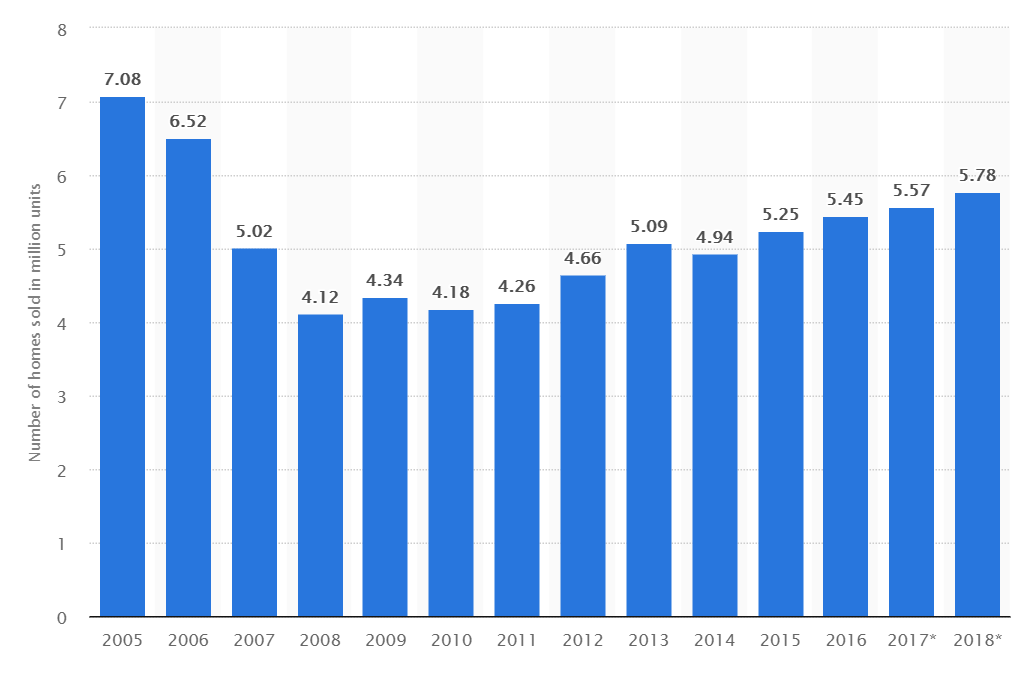
\includegraphics[width=0.8\paperwidth]{HouseSoldGraph.png}}
\end{figure}

\section{Features Description Table}
\label{appendix:Features table}
\begin{table}[H]
\centering
\resizebox{\textwidth}{!}{
\begin{tabular}{lll}
\hline
\rowcolor[HTML]{C0C0C0} 
id             & a notation for a house                                                                                                                                 & Numeric \\
date           & Date house was sold                                                                                                                                    & String  \\
\rowcolor[HTML]{C0C0C0} 
price          & Price is prediction target                                                                                                                             & Numeric \\
bedrooms       & Number of Bedrooms/House                                                                                                                               & Numeric \\
\rowcolor[HTML]{C0C0C0} 
bathrooms      & Number of bathrooms/bedrooms                                                                                                                           & Numeric \\
sqft\_living   & square footage of the home                                                                                                                             & Numeric \\
\rowcolor[HTML]{C0C0C0} 
sqft\_lot      & square footage of the lot                                                                                                                              & Numeric \\
floors         & Total floors (levels) in house                                                                                                                         & Numeric \\
\rowcolor[HTML]{C0C0C0} 
waterfront     & House which has a view to a waterfront                                                                                                                 & Numeric \\
view           & Has been viewed                                                                                                                                        & Numeric \\
\rowcolor[HTML]{C0C0C0} 
condition      & How good the condition is ( Overall )                                                                                                                  & Numeric \\
grade          & \begin{tabular}[c]{@{}l@{}}overall grade given to the housing unit, \\ based on King County grading system\end{tabular}                                & Numeric \\
\rowcolor[HTML]{C0C0C0} 
sqft\_above    & square footage of house apart from basement                                                                                                            & Numeric \\
sqft\_basement & square footage of the basement                                                                                                                         & Numeric \\
\rowcolor[HTML]{C0C0C0} 
yr\_built      & Built Year                                                                                                                                             & Numeric \\
yr\_renovated  & Year when house was renovated                                                                                                                          & Numeric \\
\rowcolor[HTML]{C0C0C0} 
zipcode        & zip                                                                                                                                                    & Numeric \\
lat            & Latitude coordinate                                                                                                                                    & Numeric \\
\rowcolor[HTML]{C0C0C0} 
long           & Longitude coordinate                                                                                                                                   & Numeric \\
sqft\_living15 & \begin{tabular}[c]{@{}l@{}}Living room area in 2015(implies-- some renovations) \\ This might or might not have affected the lotsize area\end{tabular} & Numeric \\
\rowcolor[HTML]{C0C0C0} 
sqft\_lot15    & lotSize area in 2015(implies-- some renovations)                                                                                                       & Numeric \\ \hline
\end{tabular}%
}
\caption{Dataset's features}
\end{table}
\end{appendices}

\nocite{*}
\bibliographystyle{unsrt}
\bibliography{references}
\end{document}
